%
% ---------------------------------------------------------------------
%                 Rock-Paper-Scissors FSMD Verilog/SIS Report
%              UniVR CS Architettura degli Elaboratori - 2023/24
%                                   AUTHORS:
%                           VRXXXXXX - Simone Di Maria,
%                           VRXXXXXX - Pietro Secchi
% ---------------------------------------------------------------------
%


\documentclass[a4paper,11pt]{article}
\usepackage[T1]{fontenc}
\usepackage[utf8x]{inputenc}
\usepackage[italian]{babel}
\usepackage{amsmath}
\usepackage{calc}
\usepackage[a4paper]{geometry}
\usepackage[usenames,dvipsnames]{xcolor}
\usepackage{fancyhdr} % Required for custom headers
\usepackage{lastpage} % Required to determine the last page for the footer
\usepackage{extramarks} % Required for headers and footers
%\usepackage[usenames,dvipsnames]{color} % Required for custom colors
\usepackage{graphicx} % Required to insert images
\usepackage{listings} % Required for insertion of code
\usepackage{courier} % Required for the courier font
\usepackage{pdfpages}
\usepackage{listings}
\usepackage{mdframed}
\usepackage{enumitem}
\usepackage{minted}
\usepackage{float}
\renewcommand\listingscaption{}
\newcommand\ceil[1]{\lceil#1\rceil}
\usepackage{zi4}
\usepackage{tikz}
\usetikzlibrary{automata, positioning, arrows}
\usepackage{verbatim}
\usepackage{hyperref} % Required to create hyperlinks
\usepackage{booktabs} % better tables
\usepackage{biblatex}

% Setting up hyperlinks settings
\newcommand\myshade{85}
\colorlet{mylinkcolor}{black}
\colorlet{mycitecolor}{YellowOrange}
\colorlet{myurlcolor}{Blue}
\hypersetup{
    colorlinks  = true,
    linkcolor   = mylinkcolor,
    urlcolor    = myurlcolor,
    citecolor   = mycitecolor,
    pdfpagemode = FullScreen,
}


% Setting up tikz attributes globally
\tikzset{
    ->, % makes the edges directed
    >=stealth', % makes the arrow heads bold
    node distance=5.5cm, % specifies the minimum distance between two nodes. Change if necessary.
    every state/.style={thick, fill=gray!10}, % sets the properties for each 'state' node
    initial text=play, % sets the text that appears on the start arrow
    initial distance=2.1cm,
}

\newenvironment{framescelte}[1]
  {\mdfsetup{
    frametitle={\colorbox{white}{\space#1\space}},
    innertopmargin=6pt,
    frametitleaboveskip=-\ht\strutbox,
    frametitlealignment=\center
    }
  \begin{mdframed}%
  }
  {\end{mdframed}}


% Margins
\topmargin=-0.45in
\evensidemargin=0in
\oddsidemargin=0in
\textwidth=6.25in
\textheight=9in
\headsep=0.25in

\linespread{1.1} % Line spacing


% Set up the header and footer
\pagestyle{fancy}
%\lhead{\hmwkAuthorName} % Top left header
\chead{} % Top center head
\rhead{\hmwkTitle} % Top right header
%\cfoot{} % Bottom center footer
%\rfoot{Page\ \thepage\ of\ \protect\pageref{LastPage}} % Bottom right footer
\renewcommand\headrulewidth{0.4pt} % Size of the header rule
\renewcommand\footrulewidth{0.4pt} % Size of the footer rule

%------------------------------------------------------------------------------------
%	TITOLO
%------------------------------------------------------------------------------------
%----------------------------------------------------------------------------------------
%	NAME AND CLASS SECTION
%----------------------------------------------------------------------------------------

\newcommand{\hmwkTitle}{Rock-Paper-Scissors FSMD Verilog/SIS}
\newcommand{\insertLogo}[1][2cm]{\includegraphics[width=#1]{assets/LogoUniversitàVerona.png}}
\newcommand{\hmwkClass}{Architettura degli Elaboratori}
\newcommand{\hmwkAuthorName}{Simone Di Maria (VRXXXXXX), Pietro Secchi (VRXXXXXX)}

%------------------------------------------------------------------------------------
%	TITLE PAGE
%------------------------------------------------------------------------------------

\title{
\insertLogo[8cm] \\
\vspace{0.7in}
\textmd{\textbf{\hmwkClass:\\ \hmwkTitle}}\\
\vspace{0.1in}\large{\textit{\hmwkAuthorName}}
\date{\today}
}


%\author{}

%------------------------------------------------------------------------------------


%------------------------------------------------------------------------------------
%	FORMATTAZIONE ELEMENTI
%------------------------------------------------------------------------------------
\renewcommand*{\ttdefault}{zi4}
\newcommand{\stato}[1]{\textbf{\fontfamily{zi4}\selectfont #1}}
\newcommand{\signin}[1]{\textcolor{Blue}{\fontfamily{zi4}\selectfont #1}}
\newcommand{\signout}[1]{\textcolor{BrickRed}{\fontfamily{zi4}\selectfont #1}}
\newcommand{\inctxt}[1]{\textit{\fontfamily{zi4}\selectfont #1}}
%------------------------------------------------------------------------------------


\lstdefinestyle{BashStyle}{
  language=bash,
  basicstyle=\ttfamily,
  numbers=left,
  numberstyle=\tiny\ttfamily\color{black},
  numbersep=-10pt,
  frame=tb,
  columns=fullflexible,
  title=\textit{},
  emph={souce, ps, map, -s, rl, rlib},emphstyle={\bfseries}
}

\begin{document}
  \maketitle
  \newpage
  \tableofcontents
  \newpage


\section{Specifiche del Progetto}
  Viene chiesto di realizzare il circuito di un dispositivo per la gestione di partite di Morra Cinese, noto anche come Sasso-Carta-Forbici. \\
  Il dispositivo è implementato in Verilog e SIS, due linguaggi di descrizione hardware. Il circuito riceverà in input le mosse di due player e verranno giocate da un minimo di 4 ad un massimo di 19 manche. Vince il primo giocatore che riesce a vincere due manche in più del proprio avversario, a patto di aver giocato almeno quattro manche. Si devono giocare un minimo di quattro (4) manche. Ad ogni manche, il giocatore vincente della manche precedente non può ripetere l’ultima mossa utilizzata. Nel caso lo facesse, la manche non sarebbe valida ed andrebbe ripetuta (quindi, non conteggiata). Ad ogni manche, in caso di pareggio la manche viene conteggiata. Alla manche successiva, entrambi i giocatori possono usare tutte le mosse.

\section{Struttura del progetto}
Il circuito è realizzato utilizzando il modello \textbf{{FSMD}} (Finite State Machine e Datapath) ed è quindi composto da 2 parti: un controllore relizzato tramite una Macchina a Stati Finiti (\textbf{FSM}) ed un'unità di elaborazione realizzata tramite il modello \textbf{DATAPATH}. \\
Di seguito sono riportati i pin Input/Output del circuito.
\subsection{Inputs}
  \begin{itemize}
    \item\signin{PRIMO} \inctxt{[2 bit]}: mossa scelta dal primo giocatore. Le mosse hanno i seguenti codici:
    \begin{itemize}
      \item\inctxt{00: Nessuna mossa};
      \item\inctxt{01: Sasso};
      \item\inctxt{10: Carta};
      \item\inctxt{11: Forbice};
    \end{itemize}
    
    \item\signin{SECONDO} \inctxt{[2 bit]}: mossa scelta dal secondo giocatore. Le mosse hanno gli stessi codici del primo giocatore.
    
    \item\signin{INIZIA} \inctxt{[1 bit]}: quando vale \inctxt{1}, riporta il sistema alla configurazione iniziale, considerato dunque come il segnale di "reset". Inoltre, la concatenazione degli ingressi \inctxt{PRIMO} e \inctxt{SECONDO} viene usata per specificare il numero massimo di manche oltre le quattro obbligatorie. Ad esempio, se si inserisse il valore \inctxt{PRIMO = 00} e \inctxt{SECONDO = 01}, si indicherebbe di giocare al più 5 manche (le 4 obbligatorie, più il valore \inctxt{1} indicato da \inctxt{0001}). Quando vale \inctxt{0}, la manche prosegue normalmente.
  \end{itemize}

 \newpage
  \subsection{Outputs}
  \begin{itemize}
  \item\signout{MANCHE} \inctxt{[2 bit]}: fornisce il risultato della partita con la seguente codifica:
  \begin{itemize}
      \item\inctxt{00}: La partita non è terminata;
      \item\inctxt{01}: La partita è terminata, ed ha vinto il Player 1;
      \item\inctxt{10}: La partita è terminata, ed ha vinto il Player 2;
      \item\inctxt{11}: La partita è terminata in pareggio;
    \end{itemize}
    
  \item\signout{PARTITA} \inctxt{[2 bit]}: fornisce il risultato dell’ultima manche giocata con la seguente codifica:
  \begin{itemize}
      \item\inctxt{00}: Manche non valida;
      \item\inctxt{01}: Manche vinta dal Player 1;
      \item\inctxt{10}: Manche vinta dal Player 2;
      \item\inctxt{11}: Manche pareggiata;
    \end{itemize}
  \end{itemize}

\subsection{Schematiche}
\begin{figure}[hbt!]
    \centering
    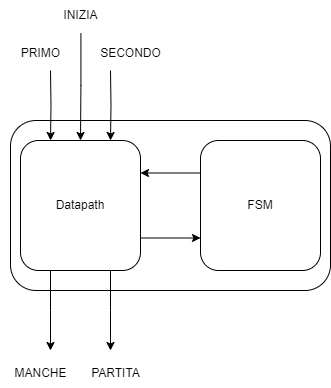
\includegraphics[width=9cm]{assets/FSM/FSDM.png}
    \caption{FSMD: Finite State Machine e Datapath}
\end{figure}

\newpage
\section{Controllore (FSM)}
Il controllore, il cui diagramma di transizione degli stati (State Transition Graph) viene riportato qui di seguito, è progettato mediante il modello Finite State Machine di Mealy. Per le scelte di design invece, si fa spesso riferimento al \cite{paper1} dei riferimenti bibliografici.

  \subsection{State Transitions Graph (STG)}
  \begin{center}
    \begin{tikzpicture}
        % States definitions here
        % \node[<options>] (name) {text label};
        \node[state, initial below,  minimum size=1.5cm] (START) {START};
        \node[state, right of=START, minimum size=1.5cm] (P1_W1) {P1 +1};
        \node[state, left  of=START, minimum size=1.5cm] (P2_W1) {P2 +1};
        \node[state, above of=P1_W1, minimum size=1.5cm] (P1_W2) {P1 +2};
        \node[state, above of=P2_W1, minimum size=1.5cm] (P2_W2) {P2 +2};

        % draw Edges
        % \draw (<source node>) edge[<edge options>] node{<edge label>} (<dest node>);
        \draw   (START) edge[loop above] node[above]{tie/idle/reset} (START)
                        edge[] node[below]{P1 win} (P1_W1)
                        edge[] node[below]{P2 win} (P2_W1)
              
                (P1_W1) edge[bend right] node[above]{P2 win/reset} (START)
                        edge[loop right] node[]{tie/idle} (P1_W1)
                        edge[] node[left]{P1 win} (P1_W2)
              
                (P2_W1) edge[bend left] node[above]{P1 win/reset} (START)
                        edge[loop left] node[]{tie/idle} (P2_W1)
                        edge[] node[right]{P2 win} (P2_W2)
                        
                (P1_W2) edge[] node[left]{P1 win/reset} (START)
                        edge[loop right] node[]{tie/idle} (P1_W2)
                        edge[bend left] node[right]{P2 win} (P1_W1)

                (P2_W2) edge[] node[right]{P2 win/reset} (START)
                        edge[loop left] node{tie/idle} (P2_W2)
                        edge[bend right] node[left]{P1 win} (P2_W1)
                        ;
    \label{STG}
    \end{tikzpicture}
  \end{center}
  Si noti l'assenza di uno stato finale. Si considera una partita terminata nel momento in cui il circuito determinerà un player vincitore. Dopodichè, viene richiesto all'utente il "reset" manuale del dispositivo. Siccome il compito dello STG è semplicemente quello di tenere traccia di quale giocatore e di quanto è in vantaggio, non è possibile determinare uno stato finale nel nostro STG. Di conseguenza, ogni stato potenzialmente è uno stato finale, in base al numero di manche giocate. Si consideri ad esempio, il caso in cui vengono giocate il numero massimo di manche, ma al momento della fine dell'ultima manche, nessun giocatore è in vantaggio di due punti, bensì uno dei due, di un solo punto. A quel punto verrà assegnata la vittoria al giocatore in vantaggio (quindi con il numero maggiore di vittorie).  
  Un'alternativa considerata durante la fase di progettazione, è stata quella di aggiungere altri due stati, \inctxt{P1\_WINNER} e \inctxt{P2\_WINNER}, rendendoli stati finali; tuttavia ciò avrebbe portato complicazioni nell'implementazione in \textit{SIS}.

\newpage
\begin{framescelte}{Scelta Progettuale n. 1}
  Si è preferito definire il \textit{STG} con l'insieme degli stati finiti (\inctxt{}F) vuoto, $F := \emptyset$. Tale scelta è stata guidata dalla volontà di utilizzare il minor numero possibile di stati, dal rendere facile l'implementazione in SIS, e dal voler mantenere il STG con il semplice compito di tenere traccia del giocatore in vantaggio.    
\end{framescelte}


  \subsection{Architettura del controllore}
Il controllore è stato progettato con il seguente diagramma di blocco per le FSM di Mealy:
 \begin{figure}[hbt!]
     \centering
     \label{fig:FSM-block-diagram}
    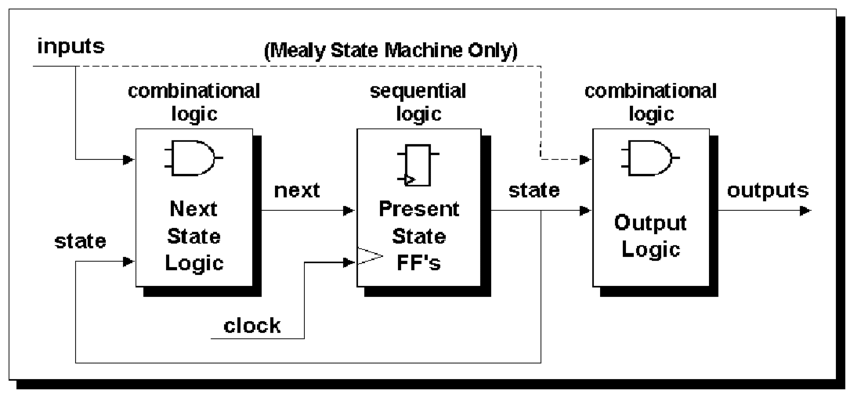
\includegraphics[width=13cm]{assets/FSM/Finite-State-Machine-FSM-block-diagram.png}
    \caption{Finite State Machine (FSM) block diagram, from \cite{paper1}}
  \end{figure}
Questa struttura ci permette di individuare due caratteristiche principali della nostra FSM:
  \begin{enumerate}
    \item \textbf{Suddivisione tra blocchi "sequenziali" e blocchi "combinatori"}: Un circuito logico combinatorio è un circuito la cui uscita dipende \textit{esclusivamente} dai suoi ingressi correnti e non ha alcuna memoria. Per questo motivo sarà anche \textit{time-insensitive}. I circuiti sequenziali, invece, sono costruiti utilizzando circuiti combinatori ed elementi di memoria chiamati “flip-flop”. Inoltre, il loro "trigger" è dato dal \inctxt{clock}, rendendoli \textit{time-sensitive}. Questi circuiti generano un output che dipende dallo stato attuale e da quello precedente. In particolare, nel nostro caso il blocco combinatorio gestirà l'esito delle manche restituendo in output, ad esempio, il prossimo stato, passandolo al blocco sequenziale che imposterà e memorizzerà lo stato corrente della macchina.

    \item \textbf{Determinazione output}: Notiamo come l'\inctxt{Output Logic} della nostra FSM [\ref{fig:FSM-block-diagram}] dipenda dallo stato attuale \textbf{e} dagli input. Di conseguenza la funzione di output della nostra FSM avrà come dominio l'insieme degli input che gli forniamo e lo stato corrente della macchina. Inoltre, deduciamo che le uscite avranno una reazione immediata agli ingressi. Nel caso la funzione di output non reagisse immediatamente alla modifica dell'inputs, e quindi dipendesse solo dallo stato corrente della macchina, staremmo parlando di FSM di Moore, e non più di Mealy.
  \end{enumerate}

\newpage
\begin{framescelte}{Scelta Progettuale n. 2}
  Si è scelto di usare come modello di FSM, la FSM di Mealy. Questa scelta caratterizza la nostra FSM nella distinzione tra blocchi sequenziali e blocchi combinatori. In particolare, il blocco combinatorio che si occupa della logica di output, sarà funzione dell'insieme di inputs e dello stato corrente. Sebbene sia possibile implementare il circuito con una FSM di Moore, la FSM di Mealy ci permette più flessibilità e semplicità nella gestione delle manche di gioco.    
\end{framescelte}

\subsection{Implementazione Verilog}
Di seguito sono riportate le principali scelte di stile e codifica prese nell'implementazione del circuito in Verilog. Per il codice completo si invita il lettore a consultare direttamente il codice sorgente poichè ben commentato.

\subsubsection{Coding Style: \textit{lowRISC Verilog Coding Style Guide}}
Nell'implementazione Verilog del circuito, si è deciso di aderire alle convenzioni elencate nella \href{https://github.com/lowRISC/style-guides/blob/master/VerilogCodingStyle.md}{lowRISC Verilog Coding Style Guide}. Tra i motivi di questa scelta è presente la volontà di scrivere codice nel modo più leggibile, coerente, pulito e standardizzato possibile per favorire la facile comprensione del codice ai lettori non-autori di questo progetto.
\begin{quote}
     \textit{To quote the Google C++ style guide: "Creating common, required idioms and patterns makes code much easier to understand."}
\end{quote}
Alcune delle "best practices" adottate nel codice sono: la \href{https://github.com/lowRISC/style-guides/blob/master/VerilogCodingStyle.md#tabular-alignment}{Tabular Alignment}, l'\href{https://github.com/lowRISC/style-guides/blob/master/VerilogCodingStyle.md#indentation}{Indentation}, il \href{https://github.com/lowRISC/style-guides/blob/master/VerilogCodingStyle.md#naming}{Naming}, la preferenza al data type \inctxt{logic}, l'uso dei costrutti \inctxt{always\_comb}, \inctxt{unique case} e \textit{blocking assignment} \inctxt{=} per la logica combinatoria, l'uso dei costrutti \inctxt{always\_ff} e \textit{non-blocking assignment} \inctxt{<=} per la logica sequenziale, etc etc.

\begin{framescelte}{Scelta Progettuale n. 3}
    Nell'implementazione del circuito in Verilog, si è deciso di seguire la \href{https://github.com/lowRISC/style-guides/blob/master/VerilogCodingStyle.md}{lowRISC Verilog Coding Style Guide} per ottenere un risultato più leggibile, coerente, pulito e standardizzato possibile e favorire la comprensione del codice ai lettori non-autori di questo progetto.
\end{framescelte}

\subsubsection{Coding Style: \textit{Two always block}}
Il "Two always block" style è una buona pratica per l'implementazione della Finite State Machine (FSM) in Verilog. Questo approccio offre una serie di vantaggi che lo rendono particolarmente adatto per questa task. In primo luogo, una priorità comune anche ad altre scelte di design prese nel corso di questo progetto, è la leggibilità del codice. Per questo motivo, utilizzare due blocchi always separati per il comportamento combinatorio (Next State Logic e Output Logic) e lo stato sequenziale (Present State FF), rende più chiaro il partizionamento delle componenti. Inoltre, questo stile di codifica aiuta a mantenere una struttura modulare e organizzata. Separando il comportamento combinatorio e lo stato sequenziale, è più semplice per il progettista concentrarsi su ciascun aspetto separatamente.
Inoltre, questo stile favorisce una migliore scalabilità e manutenibilità del codice. Se in futuro si desidera estendere o modificare la FSM per aggiungere nuovi stati o comportamenti, la separazione dei blocchi always semplifica il processo di aggiornamento del codice senza dover riscrivere completamente la logica esistente. \\
In generale il "Two always block" risulta spesso più efficace rispetto ad altri approcci come il "One always block". L'argomento è largamente discusso dal \ref{paper1} menzionato e preso in esame più volte nel corso di questo report, a cui si invita la lettura per una comprensione approfondita.
\begin{figure}
    \centering
    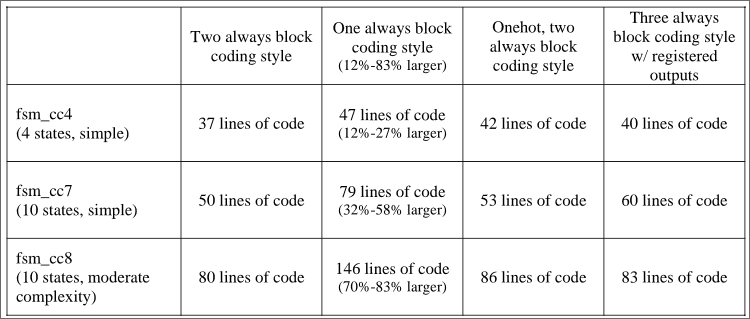
\includegraphics[width=0.9\linewidth]{assets/FSM/ComparingRTLCodingEfforts.png}
    \caption{Lines of RTL code required for different FSM coding styles, from \cite{paper1}}
\end{figure}
\begin{quote}
    \textit{The one always block FSM coding style is more verbose, more confusing and more error prone than a comparable Two always block coding style.}
\end{quote}

\begin{framescelte}{Scelta Progettuale n. 4}
    Nell'implementazione in Verilog della FSM, si è deciso di seguire il "Two always block" style, che risulta più efficace di altri approcci come il "One always block" o il "Three always block" style. 
\end{framescelte}


\subsubsection{Codifica Stati}
Per rappresentare gli stati della nostra FSM, ci siamo trovati a dover fare una scelta (non banale) sulla codifica da implementare. Una codifica adeguata per questo scopo deve essere: compatta, leggibile, e deve produrre risultati di sintesi efficienti. Tra le varie codifiche possibili, abbiamo identificato tre principali classificazioni comuni utilizzate per descrivere la codifica dello stato di una FSM: \\ 1) \textit{One-Hot Encoding (OHE)} 2) \textit{Binary Encoding} 3) \textit{Gray Code}. \\
\\
\textbf{One-Hot Encoding (OHE)}: \\
L'OHE rappresenta ciascun stato mediante un vettore binario di lunghezza pari al numero di stati possibili. In questa codifica \textbf{solo uno} dei bit del vettore che rappresenta il nostro stato è \inctxt{1}, chiamato per questo motivo "\textit{hot}". Tutti gli altri bit sono \inctxt{0}. La distanza di Hamming di questa codifica fra ogni stato è 2.
Considerando gli stati del rappresentati nel STG[\ref{STG}], la OHE li codifica come segue:

\newpage
\begin{center}
P2+2: \ \ $\begin{bmatrix} 1 \ 0 \ 0 \ 0 \ 0 \end{bmatrix}$ \\
P2+1: \ \ $\begin{bmatrix} 0 \ 1 \ 0 \ 0 \ 0 \end{bmatrix}$ \\
START:    $\begin{bmatrix} 0 \ 0 \ 1 \ 0 \ 0 \end{bmatrix}$ \\
P1+1: \ \ $\begin{bmatrix} 0 \ 0 \ 0 \ 1 \ 0 \end{bmatrix}$ \\
P1+2: \ \ $\begin{bmatrix} 0 \ 0 \ 0 \ 0 \ 1 \end{bmatrix}$ \\
\end{center}

Essendo un solo bit attivo, è necessario un solo flip-flop per ogni stato della FSM. Di conseguenza, la macchina a stati è già “decodificata”: lo stato della macchina viene determinato semplicemente leggendo quale flip-flop è attivo. Inoltre, questa codifica è più efficiente a livello di consumi rispetto alla Binary Encoding, grazie alla caratteristica di tenere solo 1 bit acceso. Questa tecnica di codifica riduce lo spazio del nostro circuito combinatorio e, di conseguenza, la macchina a stati richiede meno livelli logici tra i registri, riducendone la complessità e aumentando la velocità. \\
\\
\textbf{Binary Encoding}: \\
In questa codifica, gli stati vengono assegnati in sequenza binaria dove gli stati sono numerati a partire da \inctxt{0}. Il numero di bit $b$ necessari per codificare un numero $n$ di stati è dato dalla seguente relazione:
\begin{equation}
\label{eqn:blog2n}
    b = \ceil{\log_2{n}}
\end{equation}
Poiché la codifica binaria utilizza il numero minimo di bit (flip-flop) per codificare una macchina, i flip-flop vengono sfruttati al massimo. Di conseguenza, più logica combinatoria è necessaria per decodificare ogni stato rispetto alla OHE. Il Binary Encoding richiede meno flip-flop rispetto all'OHE, ma la distanza di Hamming può essere maggiore del numero di bit ($b$). \\
\\
\textbf{Gray Code}: \\
Il codice Gray, noto anche come codice binario riflesso, gli stati vengono assegnati in modo tale che le codifiche di stati consecutivi differiscano solo di un bit (distanza di Hamming unitaria). In questa codifica anche la relazione tra numero di bit e numero di stati è definita dalla formula[\ref{eqn:blog2n}]:
\begin{equation*}
    b = \ceil{\log_2{n}}
\end{equation*}
Il numero di flip-flop utilizzati e la complessità della logica di decodifica sono gli stessi della codifica binaria. Ma in questo caso la distanza di Hamming è sempre 1. \\
\\

\newpage\textbf{Codifiche a confronto: Pro e Contro} \\
\begin{table}[!htbp]
    \centering
    \caption{Vantaggi e Svantaggi delle varie codifiche di stato per le FSM}
    \label{tab:FSM_encoding}
    \begin{tabular}{p{3cm}p{6cm}p{6cm}}
        \toprule
        \textbf{Codifica Stati} & \textbf{Pros} & \textbf{Cons} \\
        \midrule
        \textbf{Binary Encoding} & \begin{itemize}
                            \item Richiede meno flip-flop rispetto all'encoding One Hot.
                            \item Facile da implementare e comprendere.
                            \item Adatto per FSM con pochi stati.
                         \end{itemize} 
                        & \begin{itemize}
                            \item Richiede logica extra per decodificare lo stato attuale.
                            \item Non ottimale a livello di consumo energetico.
                          \end{itemize} \\
        \textbf{One-Hot Encoding} & \begin{itemize}
                            \item Transizioni di stato dirette, nessuna necessità di decodifica.
                            \item Facile da comprendere e leggere.
                            \item Facile da estendere e modificare senza impattare altri stati.
                          \end{itemize} 
                        & \begin{itemize}
                            \item Richiede un gran numero di flip-flop.
                          \end{itemize} \\
        \textbf{Gray Code} & \begin{itemize}
                            \item Distanza di Hamming unitaria.
                            \item Riduce il consumo di potenza.
                         \end{itemize} 
                        & \begin{itemize}
                            \item Richiede logica extra per decodificare lo stato attuale.
                            \item Comprensione più complessa rispetto alla Binary Encoding e la OHE.
                            \item Non ottimale per FSM con pochi stati, poiché richiede più flip-flop rispetto all'encoding binario.
                          \end{itemize} \\
        \bottomrule
    \end{tabular}
\end{table}

\newpage
Considerando la rappresentazione degli stati con la codifica One-Hot, notiamo come potremmo sfruttare a nostro favore il "movimento" dei bit "hot". Si consideri infatti la codifica del vincitore della manche: nel caso vinca il Player 1, l'output \inctxt{MANCHE} sarà \inctxt{01}, nel caso in cui vinca Player 2, l'output \inctxt{MANCHE} sarà \inctxt{10}. Possiamo dunque aiutarci con la "direzione" del bit di \inctxt{MANCHE}, per capire verso quale direzione si muoverà la FSM e in che direzione si muoverà il bit "hot" per rappresentare il prossimo stato (\inctxt{next\_state}). \\
Ad esempio:
\begin{figure}[hbt!]
    \centering
    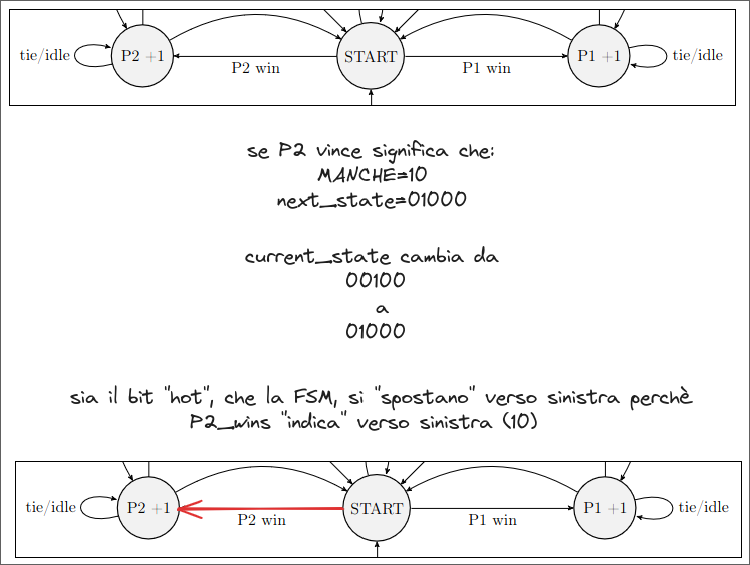
\includegraphics[width=\linewidth]{assets/FSM/bitmoving.png}
    \caption{Rappresentazione del "movimento" dei bit e della FSM al vincere di un Player}
\end{figure}

La codifica OHE, di conseguenza, aiuterebbe molto alla comprensione e alla lettura del circuito.

\newpage
\begin{framescelte}{Scelta Progettuale n. 5}
Per la codifica degli stati della FSM in Verilog è stata scelta la \textit{One-Hot Encoding}. La OHE risulta il perfetto compromesso tra leggibilità, consumi, velocità ed area utilizzata.
Per di più, secondo \cite{paper1}, questa codifica è la più coerente in contesto di progettazione FPGA:
\begin{quote}
    \textit{FPGA vendors frequently recommend using a onehot state encoding style because flip-flops are plentiful in an FPGA and the combinational logic required to implement a onehot FSM design is typically smaller than most binary encoding styles. Since FPGA performance is typically related to the combinational logic size of the FPGA design, onehot FSMs typically run faster than a binary encoded FSM with larger combinational logic blocks.}
\end{quote}
\end{framescelte}

\newpage
\section{Unità di Elaborazione}
L'unità di elaborazione è realizzata tramite il modello \textbf{\textit{datapath}}, ed è così schematizzata:
  \subsection{Datapath}
  \begin{center}
    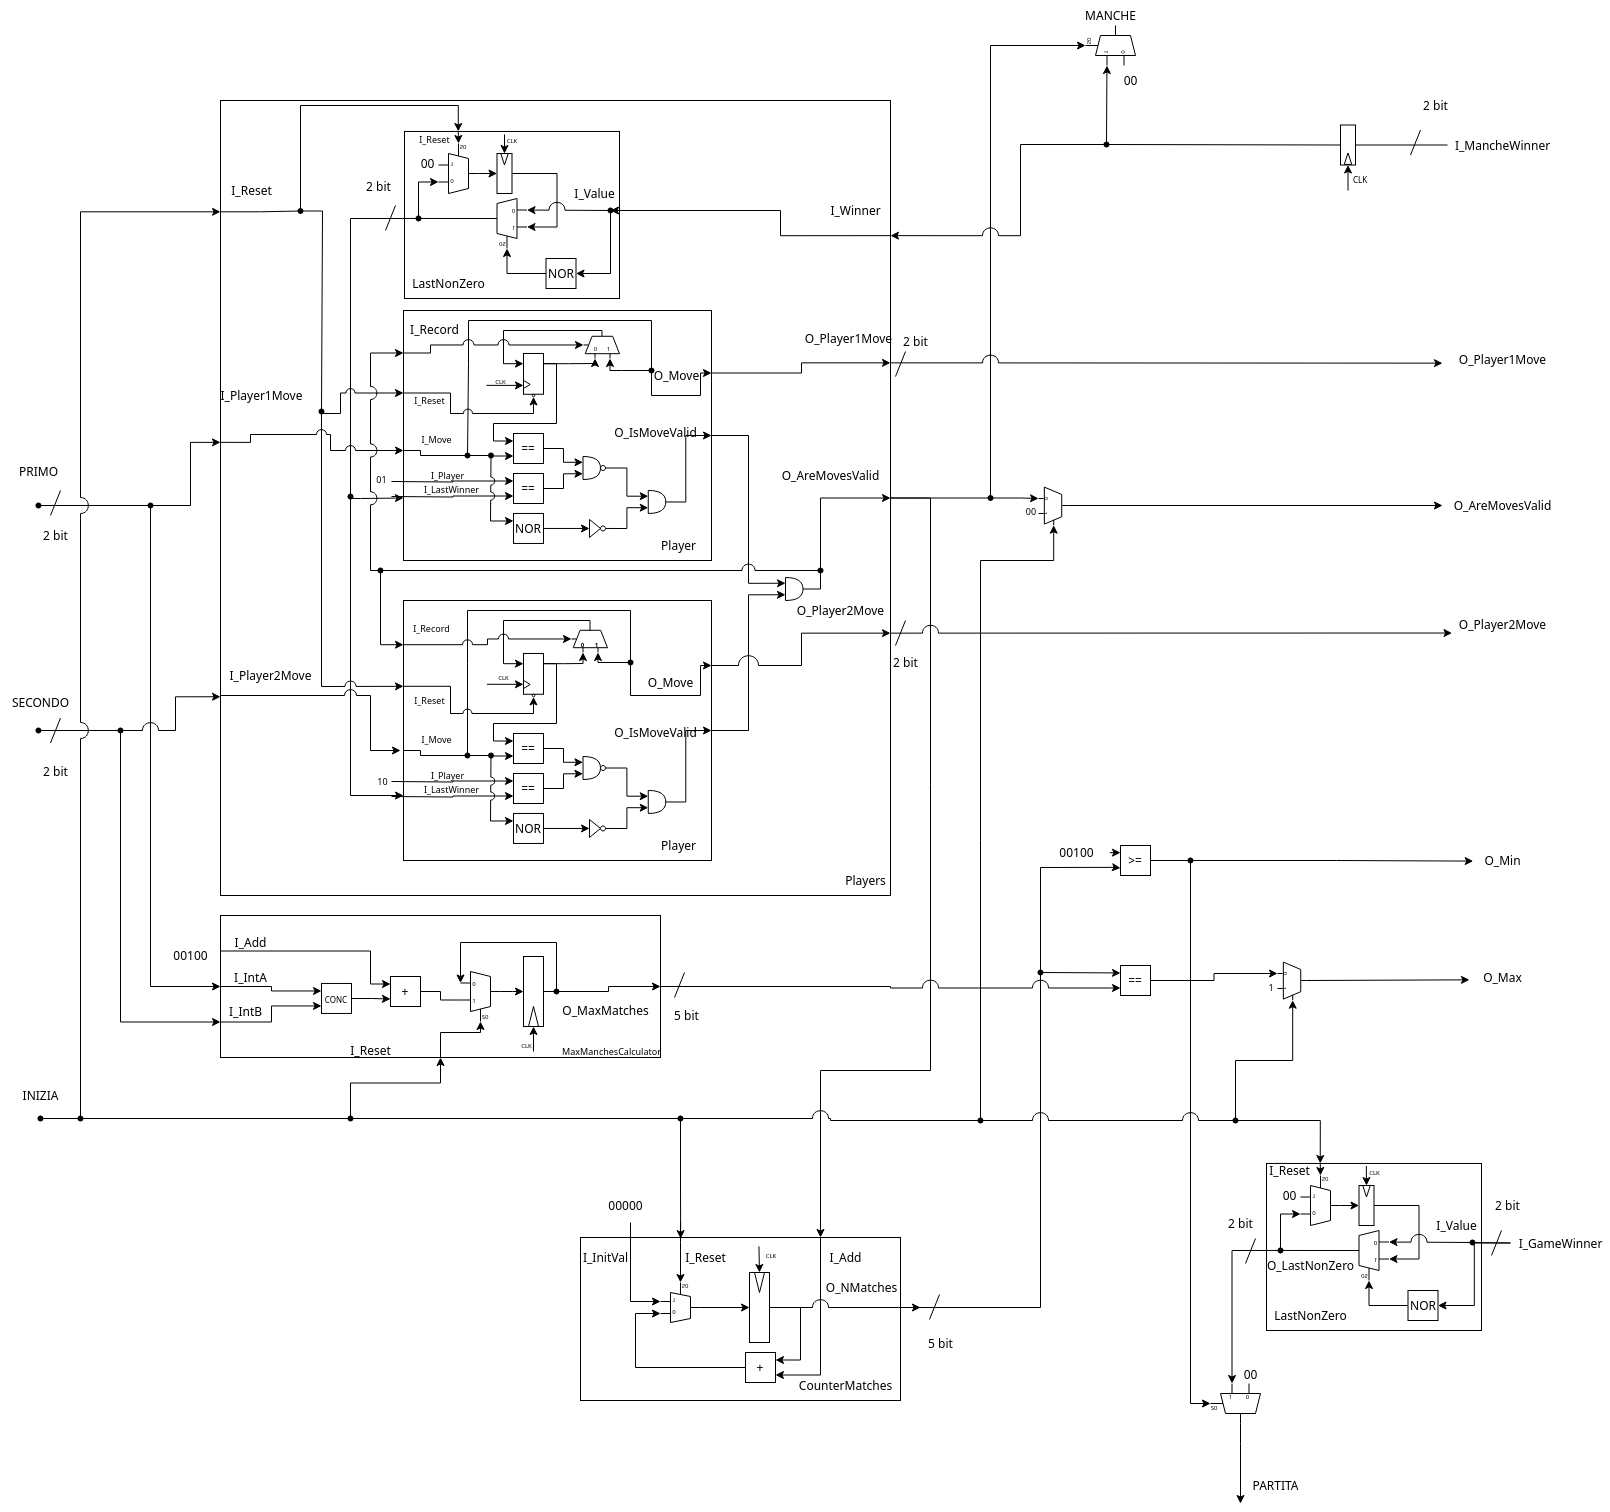
\includegraphics[width=16cm]{assets/Modules/datapath.png}
  \end{center}
Di cui si hanno 5 sottomoduli principali:

\newpage
\subsubsection{\inctxt{Player} module}
    \begin{center}
        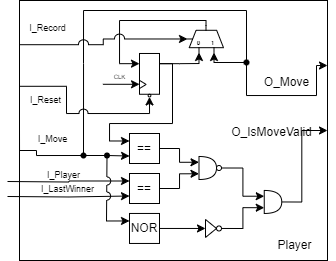
\includegraphics[width=0.6\linewidth]{assets/Modules/Player.png}
    \end{center}
    Il modulo \textbf{\inctxt{Player}} si occupa di controllare la validità delle mosse, prende in input l'ultimo vincitore, il nome del giocatore che rappresenta ($01$ o $10$), la mossa e un bit per decidere se registrare la mossa.
    Utilizza un registro \inctxt{D} con \inctxt{Reset} per resettare lo stato dell'ultima mossa in memoria.
    Per capire se la mossa è valida usa la seguente tabella di verità:

    \begin{table}[hbt!]
    \centering
    \resizebox{\columnwidth}{!}{
        \begin{tabular}{|c|c|c|c|}
            \hline
            EqualLastMove & EqualLastWinner & Invalid & $\neg$(EqualLastMove $\land$ EqualLastWinner) $\land$ $\neg$Invalid \\ \hline
            F & F & F & T \\ \hline
            F & F & T & F \\ \hline
            F & T & F & T \\ \hline
            F & T & T & F \\ \hline
            T & F & F & T \\ \hline
            T & F & T & F \\ \hline
            T & T & F & F \\ \hline
            T & T & T & F \\ \hline
        \end{tabular}
    }
    \end{table}

\newpage
\subsubsection{\inctxt{LastNonZero} module}
    \begin{center}
        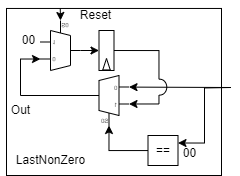
\includegraphics[width=0.5\linewidth]{assets/Modules/LastNonZero.png}
    \end{center}
    Questo modulo prende in input due bit e in output mette l'ultima coppia di bit dove entrambi non erano 0, questo viene usato in \textbf{\inctxt{Player}} per dare ai singoli player l'ultimo vincitore valido e viene usato anche per mantenere in memoria lo stato del vincitore della partita.
    Ha un bit di reset per pulire i registri.
    
\subsubsection{\inctxt{Players} module}
    \begin{center}
        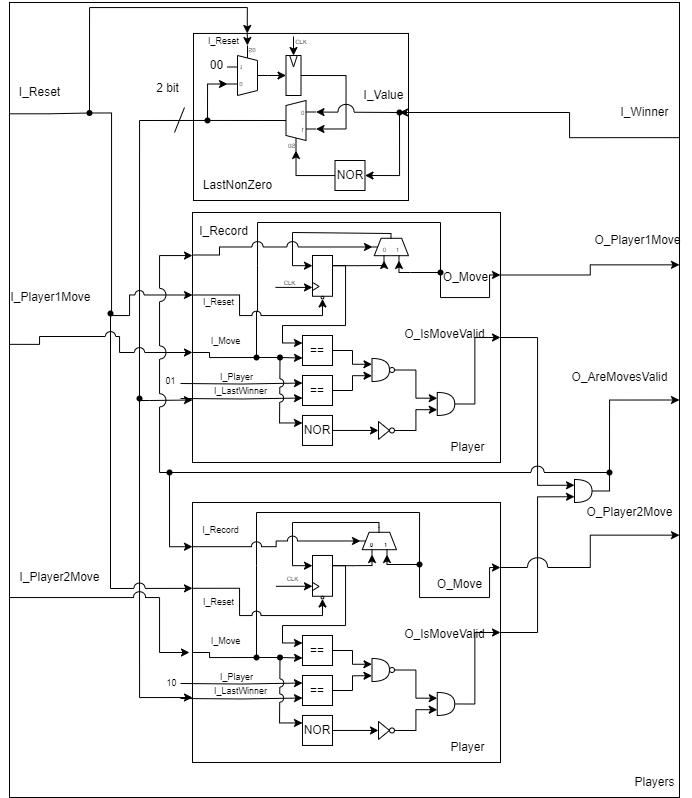
\includegraphics[width=0.75\linewidth]{assets/Modules/Players.png}
    \end{center}
    Il modulo \textbf{\inctxt{Players}} include i 2 moduli \textbf{\inctxt{Player}} e un modulo \textbf{\inctxt{LastNonZero}}, esegue un operazione di \inctxt{AND} con gli output dei \textbf{\inctxt{Player}} e il risultato viene restituito di nuovo in input ai \textbf{\inctxt{Player}} per registrare la mossa se valida (1) utilizzando un multiplexer.
    
\subsubsection{\inctxt{MaxManchesCalculator} module}
    \begin{center}
        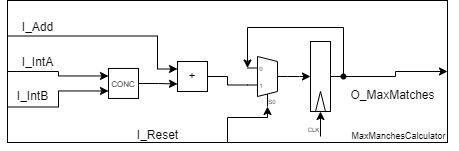
\includegraphics[width=0.6\linewidth]{assets/Modules/MaxManchesCalculator.png}
    \end{center}
    Entra in funzione quando \inctxt{INIZIA} è a 1 ed esegue una concatenazione di \inctxt{PRIMO} e \inctxt{SECONDO}, sommando poi \inctxt{I\_Add}, che in questo caso è \inctxt{00100} (4 in decimale) per avere in output il numero massimo di manche. Viene resettato con \inctxt{I\_Reset}.
    
\subsubsection{\inctxt{Counter} module}
    \begin{center}
        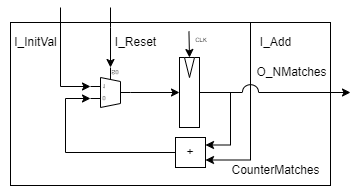
\includegraphics[width=0.6\linewidth]{assets/Modules/Counter.png}
    \end{center}
    Conta il numero di manche giocate. Il modulo prende come input \inctxt{I\_Add} che in questo caso è \inctxt{O\_AreMovesValid} di \textbf{\inctxt{Players}}, quindi se le mosse sono valide il counter viene incrementato.

\begin{framescelte}{Scelta Progettuale n. 6}
    Per risparmiare logica i controlli per confrontare un valore a \inctxt{00} vengono fatti con un operatore \inctxt{NOR}. L'input \inctxt{I\_Add} del counter di partite è direttamente \inctxt{O\_AreMovesValid} da \textbf{\inctxt{Players}}. Le mosse dei giocatori prese in input dal modulo \textbf{\inctxt{Players}} vengono passate direttamente ai moduli \textbf{\inctxt{Player}}, che le restituiranno in output sempre, anche quando non sono valide. Si sarebbe potuto far passare il segnale delle mosse senza farlo passare per i suddetti moduli; abbiamo deciso però di rendere il datapath più pulito. Il numero di manche viene registrato con registri a \inctxt{5 bit} poichè il range di valori che dobbiamo assumere è $[0, 19]$ e $\ceil{\log_2{19}} = 5$ abbiamo quindi bisogno di almeno 5 registri. Un'altra opzione sarebbe stata quella di usare un registro ad \inctxt{8 bit} perchè modulo più comune (essendo potenza di 2).
\end{framescelte}

\newpage
\section{Realizzazione del circuito in formato \inctxt{blif}}
Per poter realizzare il circuito abbiamo prima di tutto assegnato alla \textbf{FSM} - descritta sotto forma di \textbf{STG} - gli stati mediante la funzione \inctxt{state\_assign jedi}, che si è occupata anche di mappare la \textbf{FSM} come circuito sequenziale. A questo punto, valutato il corretto funzionamento rispettivamente di \textbf{FSM} e \textbf{DATAPATH}, abbiamo unito elaboratore e controllore mediante un unico file \inctxt{FSMD.blif}.

\begin{framescelte}{Warning}
    Nel caricare il file del circuito, vengono prodotti alcuni warning che indicano il mancato uso del \inctxt{COUT} di qualche modulo. Poiché questi bit non sono rilevanti, siamo riusciti a sopprimere il warning assegnando i \inctxt{COUT} ad un modulo extra che semplicemente ritorna in output quello che riceve in input, così da evitare di avere dei warning ogni volta che si carica il file \inctxt{blif}.
\end{framescelte}

\subsection{Ottimizzazione e mapping del circuito}
Siamo passati quindi all'ottimizzazione per area totale, utilizzando tutti gli script che sono disponibili all'interno della cartella di sis e questi sono i risultati per ogni comando nello script dopo diverse iterazioni:

\subsubsection{algebraic.script}
    \begin{verbatim}
    stats pre-optimization: pi= 5 po= 4 nodes=146 latches=23 lits(sop)= 819
    
    pi= 5 po= 4 nodes= 80 latches=23 lits(sop)= 617
    pi= 5 po= 4 nodes= 35 latches=23 lits(sop)= 1000
    pi= 5 po= 4 nodes= 35 latches=23 lits(sop)= 923
    pi= 5 po= 4 nodes= 35 latches=23 lits(sop)= 912
    pi= 5 po= 4 nodes= 39 latches=23 lits(sop)= 521
    pi= 5 po= 4 nodes= 39 latches=23 lits(sop)= 521
    pi= 5 po= 4 nodes= 39 latches=23 lits(sop)= 521
    pi= 5 po= 4 nodes= 39 latches=23 lits(sop)= 521
    pi= 5 po= 4 nodes= 43 latches=23 lits(sop)= 452
    pi= 5 po= 4 nodes= 43 latches=23 lits(sop)= 452
    pi= 5 po= 4 nodes= 44 latches=23 lits(sop)= 441
    pi= 5 po= 4 nodes= 44 latches=23 lits(sop)= 441
    pi= 5 po= 4 nodes= 76 latches=23 lits(sop)= 358
    pi= 5 po= 4 nodes= 76 latches=23 lits(sop)= 354
    pi= 5 po= 4 nodes= 84 latches=23 lits(sop)= 340
    pi= 5 po= 4 nodes= 84 latches=23 lits(sop)= 340
    pi= 5 po= 4 nodes= 60 latches=23 lits(sop)= 422
    
    stats post-optimization: pi= 5 po= 4 nodes= 91 latches=23 lits(sop)= 342
    \end{verbatim}
    \begin{center}
        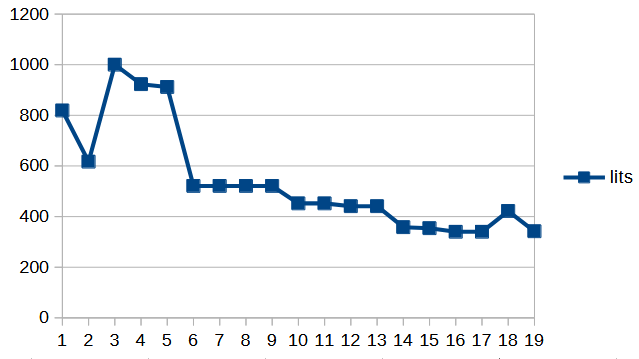
\includegraphics[width=0.5\linewidth]{assets/Charts/AlgebraicL.png}
        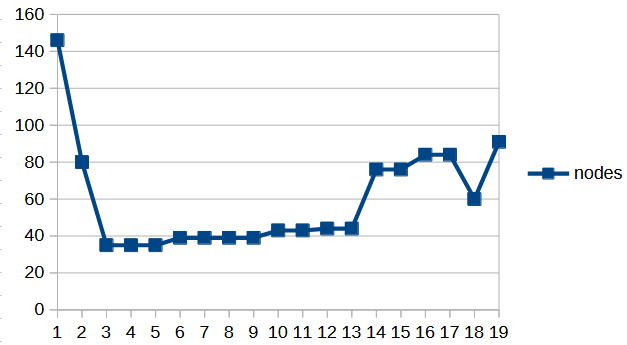
\includegraphics[width=0.5\linewidth]{assets/Charts/AlgebraicN.png}
    \end{center}

\newpage
\subsubsection{boolean.script}
    \begin{verbatim}
    stats pre-optimization: pi= 5 po= 4 nodes=146 latches=23 lits(sop)= 819
    
    pi= 5 po= 4 nodes= 45 latches=23 lits(sop)= 949
    pi= 5 po= 4 nodes= 45 latches=23 lits(sop)= 845
    pi= 5 po= 4 nodes= 43 latches=23 lits(sop)= 1055
    pi= 5 po= 4 nodes= 35 latches=23 lits(sop)= 1091
    pi= 5 po= 4 nodes= 35 latches=23 lits(sop)= 913
    pi= 5 po= 4 nodes= 35 latches=23 lits(sop)= 909
    pi= 5 po= 4 nodes= 39 latches=23 lits(sop)= 545
    pi= 5 po= 4 nodes= 39 latches=23 lits(sop)= 545
    pi= 5 po= 4 nodes= 39 latches=23 lits(sop)= 545
    pi= 5 po= 4 nodes= 39 latches=23 lits(sop)= 545
    pi= 5 po= 4 nodes= 43 latches=23 lits(sop)= 446
    pi= 5 po= 4 nodes= 43 latches=23 lits(sop)= 446
    pi= 5 po= 4 nodes= 43 latches=23 lits(sop)= 446
    pi= 5 po= 4 nodes= 43 latches=23 lits(sop)= 446
    pi= 5 po= 4 nodes= 67 latches=23 lits(sop)= 373
    pi= 5 po= 4 nodes= 67 latches=23 lits(sop)= 372
    pi= 5 po= 4 nodes= 74 latches=23 lits(sop)= 363
    pi= 5 po= 4 nodes= 74 latches=23 lits(sop)= 363
    pi= 5 po= 4 nodes= 53 latches=23 lits(sop)= 455
    pi= 5 po= 4 nodes= 92 latches=23 lits(sop)= 364
    
    stats post-optimization: pi= 5 po= 4 nodes= 57 latches=23 lits(sop)= 419
    \end{verbatim}
    \begin{center}
        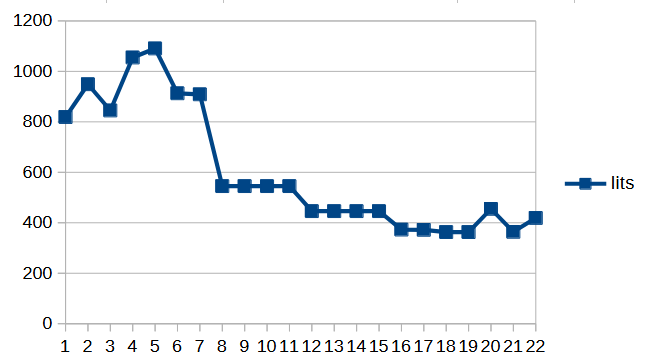
\includegraphics[width=0.6\linewidth]{assets/Charts/BooleanL.png}
        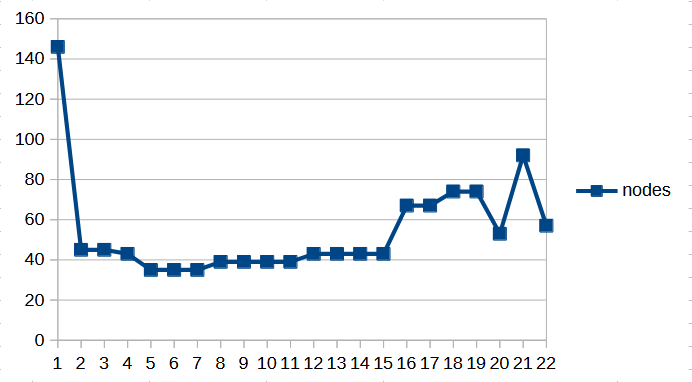
\includegraphics[width=0.6\linewidth]{assets/Charts/BooleanN.png}
    \end{center}
    
\subsubsection{delay.script}
    \begin{verbatim}
    stats pre-optimization: pi= 5 po= 4 nodes=146 latches=23 lits(sop)= 819
    
    pi= 5 po= 4 nodes= 80 latches=23 lits(sop)= 617
    pi= 5 po= 4 nodes=115 latches=23 lits(sop)= 467
    pi= 5 po= 4 nodes=367 latches=23 lits(sop)= 716
    pi= 5 po= 4 nodes=367 latches=23 lits(sop)= 634
    pi= 5 po= 4 nodes=285 latches=23 lits(sop)= 552
    
    stats post-optimization: pi= 5 po= 4 nodes= 57 latches=23 lits(sop)= 2355
    
    \end{verbatim}
    \begin{center}
        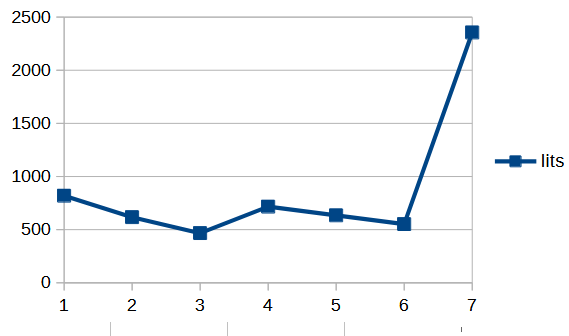
\includegraphics[width=0.6\linewidth]{assets/Charts/DelayL.png}
        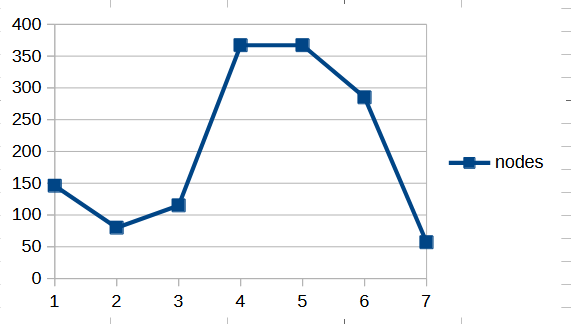
\includegraphics[width=0.6\linewidth]{assets/Charts/DelayN.png}
    \end{center}
    
\subsubsection{rugged.script}
    \begin{verbatim}
    stats pre-optimization: pi= 5 po= 4 nodes=146 latches=23 lits(sop)= 819
    
    pi= 5 po= 4 nodes= 45 latches=23 lits(sop)= 949
    pi= 5 po= 4 nodes= 45 latches=23 lits(sop)= 842
    pi= 5 po= 4 nodes= 43 latches=23 lits(sop)= 1052
    pi= 5 po= 4 nodes= 35 latches=23 lits(sop)= 1088
    pi= 5 po= 4 nodes= 35 latches=23 lits(sop)= 901
    pi= 5 po= 4 nodes= 35 latches=23 lits(sop)= 897
    pi= 5 po= 4 nodes= 77 latches=23 lits(sop)= 367
    pi= 5 po= 4 nodes= 77 latches=23 lits(sop)= 367
    pi= 5 po= 4 nodes= 56 latches=23 lits(sop)= 450
    
    stats post-optimization: pi= 5 po= 4 nodes= 56 latches=23 lits(sop)= 354
    \end{verbatim}
    \begin{center}
        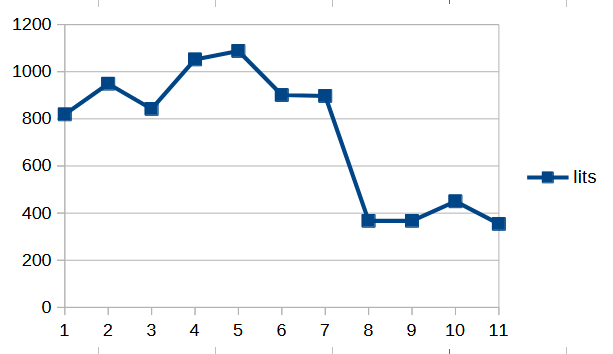
\includegraphics[width=0.6\linewidth]{assets/Charts/RuggedL.png}
        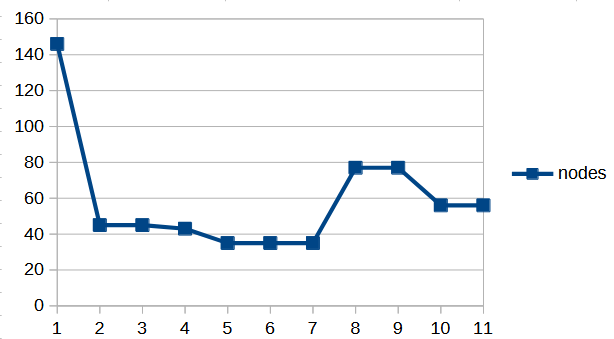
\includegraphics[width=0.6\linewidth]{assets/Charts/RuggedN.png}
    \end{center}

\newpage
\subsubsection{script}
    \begin{verbatim}
    stats pre-optimization: pi= 5 po= 4 nodes=146 latches=23 lits(sop)= 819
    
    pi= 5 po= 4 nodes= 45 latches=23 lits(sop)= 949
    pi= 5 po= 4 nodes= 45 latches=23 lits(sop)= 845
    pi= 5 po= 4 nodes= 43 latches=23 lits(sop)= 1055
    pi= 5 po= 4 nodes= 35 latches=23 lits(sop)= 1091
    pi= 5 po= 4 nodes= 35 latches=23 lits(sop)= 913
    pi= 5 po= 4 nodes= 35 latches=23 lits(sop)= 909
    pi= 5 po= 4 nodes= 39 latches=23 lits(sop)= 545
    pi= 5 po= 4 nodes= 39 latches=23 lits(sop)= 545
    pi= 5 po= 4 nodes= 39 latches=23 lits(sop)= 545
    pi= 5 po= 4 nodes= 39 latches=23 lits(sop)= 545
    pi= 5 po= 4 nodes= 43 latches=23 lits(sop)= 446
    pi= 5 po= 4 nodes= 43 latches=23 lits(sop)= 446
    pi= 5 po= 4 nodes= 43 latches=23 lits(sop)= 446
    pi= 5 po= 4 nodes= 43 latches=23 lits(sop)= 446
    pi= 5 po= 4 nodes= 67 latches=23 lits(sop)= 373
    pi= 5 po= 4 nodes= 67 latches=23 lits(sop)= 372
    pi= 5 po= 4 nodes= 74 latches=23 lits(sop)= 363
    pi= 5 po= 4 nodes= 74 latches=23 lits(sop)= 363
    pi= 5 po= 4 nodes= 53 latches=23 lits(sop)= 455
    stats post-optimization:  pi= 5 po= 4 nodes= 92 latches=23 lits(sop)= 364
    
    pi= 5 po= 4 nodes= 57 latches=23 lits(sop)= 419
    \end{verbatim}
    \begin{center}
        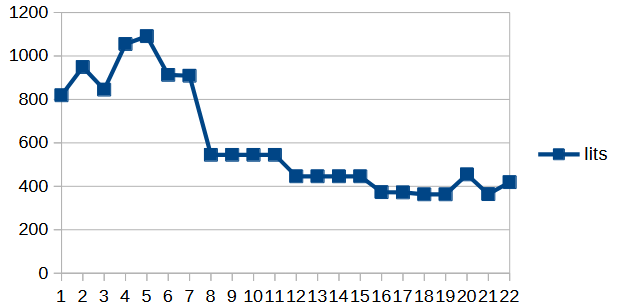
\includegraphics[width=0.6\linewidth]{assets/Charts/ScriptL.png}
        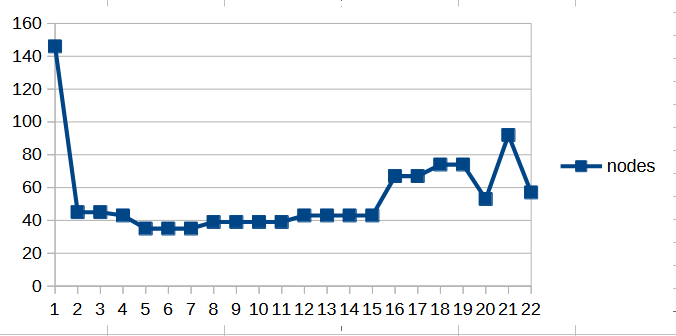
\includegraphics[width=0.6\linewidth]{assets/Charts/ScriptN.png}
    \end{center}

\begin{framescelte}{Osservazioni}
Possiamo notare che il numero di \inctxt{latch} è rimasto uguale, questo significa che abbiamo utilizzato il minimo numero di latch necessari per il progetto. \\
Possiamo anche notare che \textbf{\inctxt{script.rugged}} è stato il più performante nello semplificare i nodi, arrivando ad un numero di \inctxt{56} nodi, ma è secondo nel semplificare i letterali con un risultato di \inctxt{354} letterali, contro i \inctxt{342} di \textbf{\inctxt{algebraic.script}}.
\end{framescelte}

\newgeometry{bottom = 2.5cm, top = 1in, left = 2.5cm, right = 2.5cm}
  \subsection{Esecuzione del mapping}
  Qui di seguito viene riportato l'output dei comandi utilizzati per eseguire il mapping del progetto (dopo l'ottimizzazione) con la libreria tecnologica \inctxt{synch.genlib}.

  \begin{mdframed}[backgroundcolor=black!10]
    \begin{listing}[H]
      \begin{minted}
        [
        frame=lines,
        label = \textit{Mapping post-ottimizzazione},
        framesep=2mm,
        baselinestretch=1.2,
        bgcolor=black!10,
        fontsize=\footnotesize,
        linenos = 0
        ]
        {bash}
UC Berkeley, SIS 1.3.6 (compiled 2017-10-27 16:08:57)
sis> rl FSMD.blif
sis> print_stats
FSMD            pi= 5   po= 4   nodes=146       latches=23
lits(sop)= 819
sis> source script.rugged
sis> print_stats
FSMD            pi= 5   po= 4   nodes= 56       latches=23
lits(sop)= 354
sis>  read_library synch.genlib
sis>  map -m 0 -s
>>> before removing serial inverters <<<
# of outputs:          27
total gate area:       6248.00
maximum arrival time: (39.20,39.20)
maximum po slack:     (-4.00,-4.00)
minimum po slack:     (-39.20,-39.20)
total neg slack:      (-509.40,-509.40)
# of failing outputs:  27
>>> before removing parallel inverters <<<
# of outputs:          27
total gate area:       6120.00
maximum arrival time: (39.20,39.20)
maximum po slack:     (-4.00,-4.00)
minimum po slack:     (-39.20,-39.20)
total neg slack:      (-504.60,-504.60)
# of failing outputs:  27
# of outputs:          27
total gate area:       6024.00
maximum arrival time: (39.20,39.20)
maximum po slack:     (-4.00,-4.00)
minimum po slack:     (-39.20,-39.20)
total neg slack:      (-503.60,-503.60)
# of failing outputs:  27
sis> print_stats
FSMD            pi= 5   po= 4   nodes=152       latches=23
lits(sop)= 385
sis>
  \end{minted}
  \end{listing}
  \end{mdframed}

  \newpage
  \begin{framescelte}{Osservazioni}
  Prima di ottimizzazione e di mapping tecnologico, il circuito presentava 146 nodi e 819 letterali. Dopo l'ottimizzazione, ma prima del mapping tecnologico il circuito presentava 56 nodi e 354 letterali. Infine, post-mapping e post-ottimizzazione notiamo come i letterali aumentino rispetto all'ottimizzazione, arrivando a 152 nodi e 385 letterali.
  \end{framescelte}

\newpage
% bibliography
\begin{thebibliography}{8}
\bibitem{paper1}
Clifford E. Cummings (ICU-2002), The Fundamentals of Efficient Synthesizable Finite State Machine Design using NC-Verilog and BuildGates.

\bibitem{paper2}
Clifford E. Cummings, Heath Chambers (SNUG-2019), Finite State Machine (FSM) Design \& Synthesis using
SystemVerilog - Part I.
\end{thebibliography}

\end{document}
